\subsection{\acrlong{vi}}
When using topic models and other Bayesian models, it is computationally infeasible to compute the posterior, which means approximation is necessary. 
Approaches today use two types of inference algorithms to estimate this; sampling and optimization approaches.

A widely used sampling approach is the MCMC algorithm Gibbs sampling.
Gibbs sampling approximates the posterior distribution by trying to infer hidden structure by iteratively recalculating the state of each node based on its neighbors or similar nodes in a Bayesian network.

\gls{vi} is used to solve inference with optimization.
In \gls{vi}, we have the initial variational parameters $\nu_{init}$ in which we want approximate the true posterior distribution $p(z|\textbf{x})$ where $z$ is the hidden variables and $x$ is the observations.
We do the approximation by fitting variational parameters $\nu$, to minimize the distance between the initial distribution $v$ and $\nu^*$, where $\nu^*$ is the distribution that is closest to $p(z|\textbf{x})$.
In \autoref{fig:vi}, we can see a visualization of this where we want to optimize the variational parameters to minimize the distance to the true posterior distribution.
In \autoref{fig:vi}, $q(z; \nu)$ is a family of variational distributions over the latent variables which are different instances of the hidden variables $z$.
Our goal is to fit the variational parameters $\nu$ to estimate the hidden variables that are closest to $p(z|\textbf{x})$

\begin{figure}
	\centering
	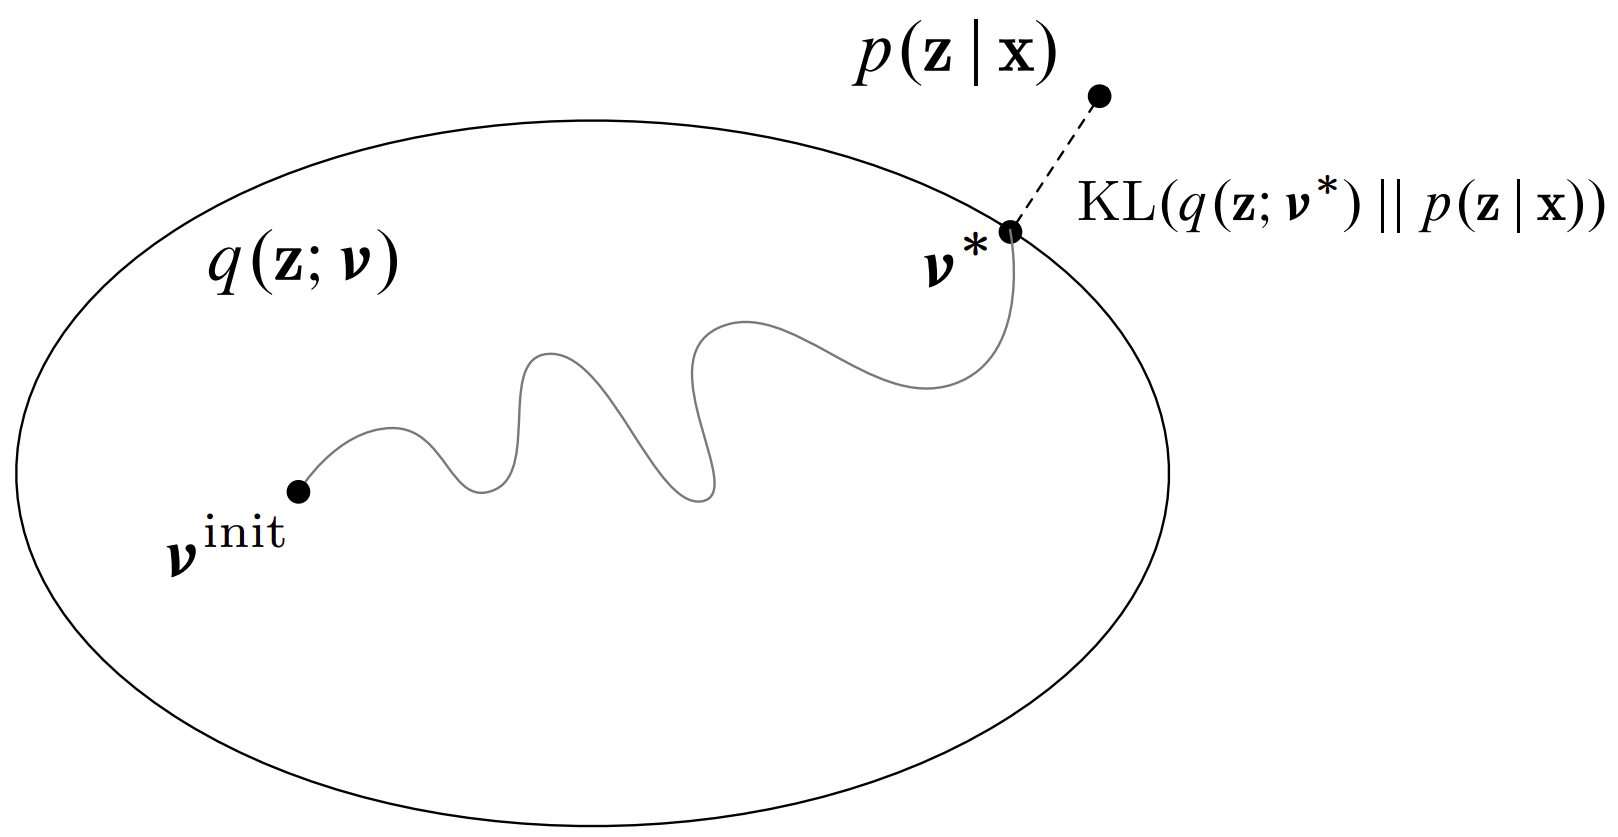
\includegraphics[width=0.5\textwidth]{figures/vi_illustration.png}
	\caption[Caption for LOF]{Illustration of \acrlong{vi}\footnotemark.}
	\label{fig:vi}
\end{figure}
\footnotetext{http://www.cs.columbia.edu/~blei/talks/Blei\_VI\_tutorial.pdf}

\subsubsection*{LDA learning}
We use an implementation of the \gls{lda} which is based on \cite{blei2010online}, where \citeauthor{blei2010online} present a way of training the \gls{lda} using \gls{vi}.
They do this by using stochastic \gls{vi}, which also outperforms batch learning.
In learning the \gls{lda}, we first sample a batch of documents from the whole corpus, where we learn the structure of this sample and use it to update the topics within the model.
To do this, we need some form of verification of whether we are getting closer to the the true posterior distribution $p(z|\textbf{x})$.
In \gls{lda}, we use perplexity as a score to check whether we are moving towards $p(z|\textbf{x})$
